% Options for packages loaded elsewhere
\PassOptionsToPackage{unicode}{hyperref}
\PassOptionsToPackage{hyphens}{url}
\documentclass[
  12pt,
]{article}
\usepackage{xcolor}
\usepackage[margin=1in]{geometry}
\usepackage{amsmath,amssymb}
\setcounter{secnumdepth}{5}
\usepackage{iftex}
\ifPDFTeX
  \usepackage[T1]{fontenc}
  \usepackage[utf8]{inputenc}
  \usepackage{textcomp} % provide euro and other symbols
\else % if luatex or xetex
  \usepackage{unicode-math} % this also loads fontspec
  \defaultfontfeatures{Scale=MatchLowercase}
  \defaultfontfeatures[\rmfamily]{Ligatures=TeX,Scale=1}
\fi
\usepackage{lmodern}
\ifPDFTeX\else
  % xetex/luatex font selection
\fi
% Use upquote if available, for straight quotes in verbatim environments
\IfFileExists{upquote.sty}{\usepackage{upquote}}{}
\IfFileExists{microtype.sty}{% use microtype if available
  \usepackage[]{microtype}
  \UseMicrotypeSet[protrusion]{basicmath} % disable protrusion for tt fonts
}{}
\makeatletter
\@ifundefined{KOMAClassName}{% if non-KOMA class
  \IfFileExists{parskip.sty}{%
    \usepackage{parskip}
  }{% else
    \setlength{\parindent}{0pt}
    \setlength{\parskip}{6pt plus 2pt minus 1pt}}
}{% if KOMA class
  \KOMAoptions{parskip=half}}
\makeatother
\usepackage{graphicx}
\makeatletter
\newsavebox\pandoc@box
\newcommand*\pandocbounded[1]{% scales image to fit in text height/width
  \sbox\pandoc@box{#1}%
  \Gscale@div\@tempa{\textheight}{\dimexpr\ht\pandoc@box+\dp\pandoc@box\relax}%
  \Gscale@div\@tempb{\linewidth}{\wd\pandoc@box}%
  \ifdim\@tempb\p@<\@tempa\p@\let\@tempa\@tempb\fi% select the smaller of both
  \ifdim\@tempa\p@<\p@\scalebox{\@tempa}{\usebox\pandoc@box}%
  \else\usebox{\pandoc@box}%
  \fi%
}
% Set default figure placement to htbp
\def\fps@figure{htbp}
\makeatother
% definitions for citeproc citations
\NewDocumentCommand\citeproctext{}{}
\NewDocumentCommand\citeproc{mm}{%
  \begingroup\def\citeproctext{#2}\cite{#1}\endgroup}
\makeatletter
 % allow citations to break across lines
 \let\@cite@ofmt\@firstofone
 % avoid brackets around text for \cite:
 \def\@biblabel#1{}
 \def\@cite#1#2{{#1\if@tempswa , #2\fi}}
\makeatother
\newlength{\cslhangindent}
\setlength{\cslhangindent}{1.5em}
\newlength{\csllabelwidth}
\setlength{\csllabelwidth}{3em}
\newenvironment{CSLReferences}[2] % #1 hanging-indent, #2 entry-spacing
 {\begin{list}{}{%
  \setlength{\itemindent}{0pt}
  \setlength{\leftmargin}{0pt}
  \setlength{\parsep}{0pt}
  % turn on hanging indent if param 1 is 1
  \ifodd #1
   \setlength{\leftmargin}{\cslhangindent}
   \setlength{\itemindent}{-1\cslhangindent}
  \fi
  % set entry spacing
  \setlength{\itemsep}{#2\baselineskip}}}
 {\end{list}}
\usepackage{calc}
\newcommand{\CSLBlock}[1]{\hfill\break\parbox[t]{\linewidth}{\strut\ignorespaces#1\strut}}
\newcommand{\CSLLeftMargin}[1]{\parbox[t]{\csllabelwidth}{\strut#1\strut}}
\newcommand{\CSLRightInline}[1]{\parbox[t]{\linewidth - \csllabelwidth}{\strut#1\strut}}
\newcommand{\CSLIndent}[1]{\hspace{\cslhangindent}#1}
\setlength{\emergencystretch}{3em} % prevent overfull lines
\providecommand{\tightlist}{%
  \setlength{\itemsep}{0pt}\setlength{\parskip}{0pt}}
% The caption filter emits genuine table floats. Declare the table packages
% explicitly because Pandoc sees those floats as raw LaTeX rather than tables.
\usepackage{longtable,booktabs,array,calc}
% Captions already contain their manuscript numbers. Keep the text at body size
% while suppressing duplicate automatic Figure/Table labels.
\usepackage{caption}
\captionsetup{labelformat=empty,font=normalsize,justification=raggedright,singlelinecheck=false}
\captionsetup[longtable]{width=\linewidth}
\usepackage{pdflscape}
\usepackage[section]{placeins}
% Pandoc emits both width and height bounds; graphicx must preserve aspect ratio.
\setkeys{Gin}{keepaspectratio}
% Inline 'h' floats can overfill pages shared with longtable's output routine.
\makeatletter
\def\fps@figure{tbp}
% Include the final line's math/subscript depth in the page-height budget.
% Otherwise TeX can place descenders below the nominal one-inch bottom margin.
\maxdepth=0pt
\@maxdepth=0pt
\makeatother
\usepackage{bookmark}
\IfFileExists{xurl.sty}{\usepackage{xurl}}{} % add URL line breaks if available
\urlstyle{same}
\hypersetup{
  pdftitle={Coalition Deception and Defensive Adaptation in a Social-Deduction Benchmark},
  pdfauthor={Isaac Lin; Xi Chen},
  pdfkeywords={multi-agent reinforcement learning, learning
dynamics, strategic communication, robust aggregation, partial
observability},
  hidelinks,
  pdfcreator={LaTeX via pandoc}}

\title{Coalition Deception and Defensive Adaptation in a
Social-Deduction Benchmark}
\author{Isaac Lin \and Xi Chen}
\date{}

\begin{document}
\maketitle
\begin{abstract}
How well do defenses against coordinated testimony withstand attackers
trained against them? We investigate a social-deduction benchmark with
structured claims, exact truth labels, and two impostors sharing a
reinforcement-learning policy. An exploratory 240-job study finds higher
false-ejection rates and raw vote agreement after training; this does
not establish communication-driven collusion. With five crew and two
impostors, descriptive multi-round coalition-victory rates are 0.967
before defender training, 0.360 afterward, and 0.851 after coalition
retraining. Training optimizes victory, while innocent ejections remain
frequent. Ten-generation crossplay shows renewed gains against the
latest opponent, without establishing an asymptotic cycle. A
hypothesis-based defender incurs substantial truthful-testimony error
and is vulnerable to targeted training, which increases false ejection
from 0.126 to 0.422. Ballot diagnostics support an abstention-related
vulnerability under fixed recorded votes. Scripted alibi errors occur
without excessive total coalition credibility weight, but scoring
interventions do not identify a unique causal channel. A separate
Gaussian surrogate characterizes when weight amplification is possible
under explicit assumptions. Dependence penalties have mixed effects on
victory and voting harm. These findings support evaluating defenses
across adaptive opponents, distinct outcomes, and directly measured
mechanisms.
\end{abstract}

\FloatBarrier

\section{Introduction}\label{introduction}

In social deduction, players combine private observations and public
testimony to decide whom to eject. Agreement can reflect independent
evidence or coordination within a hidden coalition. A defense that
handles a scripted alibi may therefore perform differently against an
adversary trained to exploit its decisions.

We study this problem in an Among Us-inspired benchmark with two
policy-sharing impostors, structured claims, and explicit records of
evidence, testimony, and votes. The benchmark supports both scripted
attacks and learned responses. Our question is how defensive performance
changes with the attacker, the training sequence, and the definition of
harm.

Strategic communication connects to cheap-talk and signaling games
\citeproc{ref-crawford1982}{{[}1{]}}, \citeproc{ref-lewis1969}{{[}2{]}},
trainable sender--receiver systems
\citeproc{ref-kharitonov2019}{{[}3{]}},
\citeproc{ref-condorelli2024}{{[}4{]}}, and information aggregation with
multiple senders \citeproc{ref-chen2025}{{[}5{]}},
\citeproc{ref-arieli2023}{{[}6{]}}. Robust aggregation,
Byzantine-resilient reinforcement learning, and peer prediction offer
related defenses with explicit assumptions
\citeproc{ref-arieli2023}{{[}6{]}}, \citeproc{ref-figura2021}{{[}7{]}},
\citeproc{ref-witkowski2012}{{[}8{]}}; geometric-median mechanisms also
face strategyproofness limits \citeproc{ref-elmhamdi2023}{{[}9{]}}.
Learned social-deduction agents and Among Us-style communication have
already been studied \citeproc{ref-kopparapu2022}{{[}10{]}},
\citeproc{ref-sarkar2025}{{[}11{]}}. Adversarial communication, credit
assignment, cooperation under uncertain incentives, and secret collusion
provide adjacent settings \citeproc{ref-blumenkamp2021}{{[}12{]}},
\citeproc{ref-li2021}{{[}13{]}}, \citeproc{ref-orzan2024}{{[}14{]}},
\citeproc{ref-motwani2024}{{[}15{]}}.

Adaptive evaluation is already an established requirement in adversarial
robustness \citeproc{ref-tramer2020}{{[}16{]}}, as is learning
approximate responses to policy populations
\citeproc{ref-lanctot2017}{{[}17{]}}. Our contribution is the
combination of adaptive-defense crossplay, separate victory and
innocent-harm outcomes, and direct diagnostics of testimony scores and
ballots in one structured benchmark. Claim labels describe testimony
alongside voting outcomes; crossplay distinguishes opponent-specific
gains from transfer. A Gaussian report model supplies a separate,
analytically tractable account of weight amplification.

The results are exploratory and do not support a single ranking of
defenses. Scripted benefits coexist with baseline errors and targeted
vulnerability. Training objectives also differ from some evaluated
harms, so improved reward does not imply uniformly better defensive
decisions.

\FloatBarrier

\section{Methods}\label{methods}

\FloatBarrier

\subsection{Benchmark and information}\label{benchmark-and-information}

The benchmark contains two hidden impostors and 3, 5, or 7 crew members,
denoted 3+2, 5+2, and 7+2. Roles are randomized each episode. A meeting
consists of structured claims, responses, and a plurality vote among
non-skip candidate ballots. Skip ballots are excluded from the tally:
the unique candidate with the most votes is ejected even if most voters
skip. No candidate ballots, or a tie for the highest candidate tally,
produces no ejection. Ejection does not reveal roles. The incident time
is public. The two impostors share a policy, reward, and a feature
identifying their partner. Unless ablated, spatial policies also
exchange private four-symbol messages.

The meeting-only configuration (F1--F2) generates private evidence
through six random-walk steps on the Hub--Electrical, Hub--Navigation,
and Hub--Medbay star map, with stay probability 0.35 and one exogenously
placed incident. The spatial configuration uses the same rooms plus an
Electrical--Navigation edge, eight movement steps, and two tasks per
agent. An impostor can create an incident only with one crew target and
no other living crew in the room; its partner may be present. Spatial
experiments use either one meeting or up to eight rounds. These
configurations differ in evidence generation, map, and communication, so
their comparison does not isolate attack adaptation.

Players see their own evidence and the public transcript. Scripted
policies use their permitted within-round positive and negative
sightings; learned spatial actors receive the corresponding time-indexed
private-history block, without unseen or future positions. Scripted
movement uses only available observations. Role-blind incident masks and
legal no-op attempts prevent action availability from revealing the
partner in hidden-identity controls. Claims receive exact true,
unsupported, false, or contradictory labels from recorded states and
speaker evidence. No-information is a separate action, not a truth
label.

\FloatBarrier

\subsection{Testimony and defenses}\label{testimony-and-defenses}

Scripted crew choose informative supported claims and use the same
suspicion rule for responses and votes. F2 compares four coalition
scripts: supported testimony; a lone creator lying about its location; a
creator's false self-alibi supported by its partner; and joint
scene-placement claims framing an innocent. The latter two coordinate
responses and votes; without a channel, their alibi rooms need not
agree. Supported testimony still allows selective disclosure and
coalition-protective voting. These scripts differ in several behaviors,
rather than manipulating agreement alone.

For voter \(v\) and candidate \(j\), ordinary rules combine private
evidence and speaker-specific testimony:

\[
S_v(j)=\mathrm{own}_v(j)+\operatorname{AGG}_s[\mathrm{signal}_v(s,j)].
\]

Scene-placement claims and accusations increase suspicion; witness
alibis reduce it. Personally detected lies penalize their speaker within
that speaker's row. The rules use an unweighted sum (called mean), a
rescaled median or trimmed mean, or credibility-weighted sums.
Credibility is −3 for a caught lie, otherwise −2 for self-contradiction,
otherwise the count of compatible informative speakers. Softmax
temperatures are 1.5 (soft) and 0.15 (sharp).

Dependence-aware credibility multiplies soft weights by
\(e^{-4\mathrm{ex}_s}\), where \(\mathrm{ex}_s\) measures agreement with
a speaker's closest partner beyond its average agreement. It pools claim
compatibility, alibis, supportive responses, and aligned non-skip votes
over three meetings. The ballot variant discounts votes and remains
active with learned crew.

The hypothesis rule enumerates two-member coalitions, excluding publicly
known crew, and averages constraint feasibility over honesty gates and
auxiliary creator/time assignments. Each coalition speaker's informative
claims are accepted with probability one half or ignored. Infeasible
hypotheses receive zero weight; positive scores are normalized. Voting
requires membership score above one half, with lexicographic ties
resolved by creator score, private evidence, then agent index; all-zero
views abstain when legal. The solver checks emitted constraints, with a
necessary-constraint relaxation for some negative transition claims.
These are heuristic feasibility scores, not calibrated generative
posteriors. Appendix B lists suspicion coefficients; public
configurations specify the complete actions and policies.

\FloatBarrier

\subsection{Training and experimental
design}\label{training-and-experimental-design}

Masked, non-recurrent actor--critic policies use PPO
\citeproc{ref-schulman2017}{{[}18{]}},
\citeproc{ref-huang2022}{{[}19{]}} with two 128-unit hidden layers,
learning rate \(3\times10^{-4}\), discount 1, GAE parameter 0.95, clip
0.2, four phase-stratified minibatches, and up to eight epochs.
Approximate KL above 0.075 stops an update; the value coefficient and
gradient-norm limit are 0.5, and the entropy coefficient declines from
0.02 to 0.005. Standard stages train for 400 updates. Each update
collects complete batches of 64 episodes in F1 or 32 in spatial
experiments. Unfinished trajectories are never finalized with terminal
targets. Evaluation uses a copied policy and independent action
randomness.

Rewards are terminal and do not directly reward lying or coordination.
F1 gives the coalition +1 for an innocent ejection after a real incident
and −1 otherwise. F3's zero-sum balanced-ejection objective gives the
coalition +1 for innocent ejection, 0 for no ejection, and −1 for
coalition ejection after a real incident. Without an incident it gives
the coalition −1 and the crew +1 regardless of the vote, including an
innocent ejection. Thus incident-free voting harm is unpenalized by this
objective. Single-meeting multigeneration loops retain that coalition
objective but train crew with meeting-ejection rewards after a real
incident: +1 for coalition ejection, −1 for innocent ejection, and 0 for
no ejection or no incident. Reward controls compare these constructions.
In multiround survival experiments, the coalition wins when living
impostors are at least as numerous as living crew after a meeting vote;
crew win by eliminating the coalition or reaching the round cap without
that condition. This reward optimizes victory, not avoidance of innocent
ejections. A separate control substitutes the incident-gated
innocent-ejection count for survival.

Response training proceeds \(C_0\rightarrow D_1\rightarrow C_1\):
coalition against scripted soft-credibility crew, crew against frozen
\(C_0\), then coalition against frozen \(D_1\). Every stage starts fresh
actor and critic weights. Multigeneration loops continue these
approximate responses with matched seed offsets and budgets. They do not
track a continuously updated policy. Crossplay tests frozen policies;
policy distances use fixed probe observations and include initialization
effects.

The corrected study comprises 240 jobs and 1,255 learner stages:

\FloatBarrier

\begin{table}[htbp]
\centering
\caption{Table 1. Study cohorts and evaluation budgets. Episodes and generations
are repeated observations within a seed or evaluation replicate;
complete job definitions and comparison expressions are versioned with
the data.}\label{tab:1}
\begin{tabular}{@{}
  >{\raggedright\arraybackslash}p{(\linewidth - 2\tabcolsep) * \real{0.2300}}
  >{\raggedright\arraybackslash}p{(\linewidth - 2\tabcolsep) * \real{0.7700}}@{}}
\toprule\noalign{}
\begin{minipage}[b]{\linewidth}\raggedright
Experiment
\end{minipage} & \begin{minipage}[b]{\linewidth}\raggedright
Independent units and evaluation budget
\end{minipage} \\
\midrule\noalign{}

F1 & Ten training seeds per population; 400 holdout episodes at
genuinely untrained and final checkpoints. \\
F2 & Ten evaluation replicates; 1,000 episodes per
rule/condition/population. \\
F3--F4 & Ten seeds per population; 1,000 final episodes for each of four
pairings. \\
Multigeneration & Ten seeds through ten generations for 5+2 in both
regimes and 3+2 multiround; five seeds through three generations for 7+2
multiround. Each stage uses 1,000 episodes; full crossplay uses 500 per
cell. \\
Defended loop & Ten seeds and four generations. \\
Adaptive defenses & Ten seeds at 5+2; five at 3+2 for dependence defense
and at 7+2 for hypothesis defense. \\
Static spatial studies and controls & Five seeds; information,
defender-budget, and reward controls use matched reference seeds. \\
\bottomrule\noalign{}
\end{tabular}
\end{table}

Controls remove partner identity, the private channel, or both; increase
defender training to 800 or 1,600 updates where specified; and replace
single-meeting or multiround rewards. Complete designs, cohorts, and
signed comparisons are versioned with the data.

\FloatBarrier

\subsection{Outcomes, inclusion, and
inference}\label{outcomes-inclusion-and-inference}

For learned experiments, the independent unit is a training seed; for
scripted experiments, it is an independently seeded evaluation batch.
Episodes and generations are repeated observations. Every planned job
passed checks of source, configuration, checkpoints, and raw records. No
seed was removed or stopped for its outcome. Historical experiments,
incomplete runs, and engineering smoke tests are excluded. Several
implementation components changed together; historical differences
cannot identify an isolated repair's effect.

Single-meeting outcomes include false ejection, creator ejection, no
ejection, and incident probability. Creator ejection and survival
require an incident and are not unconditional complements. Multiround
outcomes distinguish coalition victory, any innocent ejection, and mean
innocent-ejection count. Whole-game records include every completed
meeting, including incident-free meetings; terminal-meeting and pooled
per-meeting rates remain separate. Dependence records retain the
pre-ejection electorate and count historical meetings once. Conditional
metrics are averaged over seeds with nonzero denominators, retaining
contributing counts; undefined values are not replaced by zero.

Aligned voting is the fraction of meetings with both coalition ballots
recorded in which both choose the same non-skip target; any skip counts
as nonalignment. Multiround games use the terminal meeting. This raw
agreement rate has no matched-independent baseline. The false-claim
fraction counts claims labelled FALSE among all coalition claim actions,
including non-informative claims.

Final evaluation starts at seed 1987654321 plus run seed, separately
from monitoring at 987654321 plus run seed, and does not advance
training randomness. Predetermined episode indices are completed without
selecting faster games. F2 pairs replicate identities, while its
rule/condition-specific streams do not hold evidence or complete
transcripts fixed.

For 303 specified contrasts in 15 families, matched seed outcomes are
subtracted before calculating mean effects, sample SDs, and pointwise
95\% percentile intervals from 20,000 resamples of complete seed
differences. Two-sided exact sign-flip tests preserve magnitudes and
require null sign symmetry/exchangeability; pairing alone does not
establish that assumption. Holm correction applies within each declared
family. All contrasts, including unfavorable and nonsignificant results,
are released. This post-audit specification was not prospective
preregistration of the original research.

The minimum raw two-sided p-value is 0.001953125 with ten seeds and
0.0625 with five. Thus five-seed tests cannot reject at 0.05, nor can a
ten-seed family with at least 26 tests pass Holm's first threshold.
Families were retained despite this limit. With five seeds, only 126
distinct bootstrap seed-count multisets are possible; their intervals
are descriptive. Intervals are not simultaneous, and nonrejection does
not establish equivalence. Unqualified numerical comparisons are
descriptive means and sample SDs.

\FloatBarrier

\subsection{Mechanism diagnostics and response
gaps}\label{mechanism-diagnostics-and-response-gaps}

The descriptive mechanism study evaluates 540,000 episodes: ten
replicates per population, four scripts, and nine rule/variant cells,
with 500 episodes each. Cells within a condition share initial evidence;
responses and votes can change. The descriptive ballot study evaluates
retained hypothesis-attack checkpoints in 135 cells of 500 episodes,
using ten seeds at 5+2 and five at 7+2. Removing ballots holds other
recorded votes fixed and does not estimate behavioral adaptation.

For crossplay matrix \(M\), the exploratory finite-pool gap
\(G_k=\max_iM_{ik}-\min_jM_{kj}\) includes later-trained policies.
Simultaneous Hoeffding bands account for cell uncertainty and selection
of extrema, assuming independent episode draws within each cell. This
retrospective gap is neither true exploitability nor a convergence test.

\FloatBarrier

\section{Results}\label{results}

\FloatBarrier

\subsection{False ejection and vote agreement after
training}\label{false-ejection-and-vote-agreement-after-training}

In the meeting-only game (F1), coalition training increases false
ejection from 0.045 to 0.271 at 3+2, from 0.073 to 0.2125 at 5+2, and
from 0.091 to 0.194 at 7+2. All three final-minus-untrained contrasts
have Holm-adjusted \(p=0.0117\) in the six-test F1 family. Raw
same-target vote agreement and creator survival also increase, while the
fraction of claim actions labelled FALSE decreases at every population
(Figure 1). At 5+2, vote agreement rises from 0.108 to 0.316 and the
false-claim fraction falls from 0.423 to 0.349. Shared policy
parameters, public observations, and incentives can produce aligned
votes without communication-driven collusion; no matched-independent
learned-policy baseline is reported. Because non-informative actions
enter its denominator, the lower false-claim fraction does not establish
greater truthfulness among informative claims.

\begin{figure}
\centering
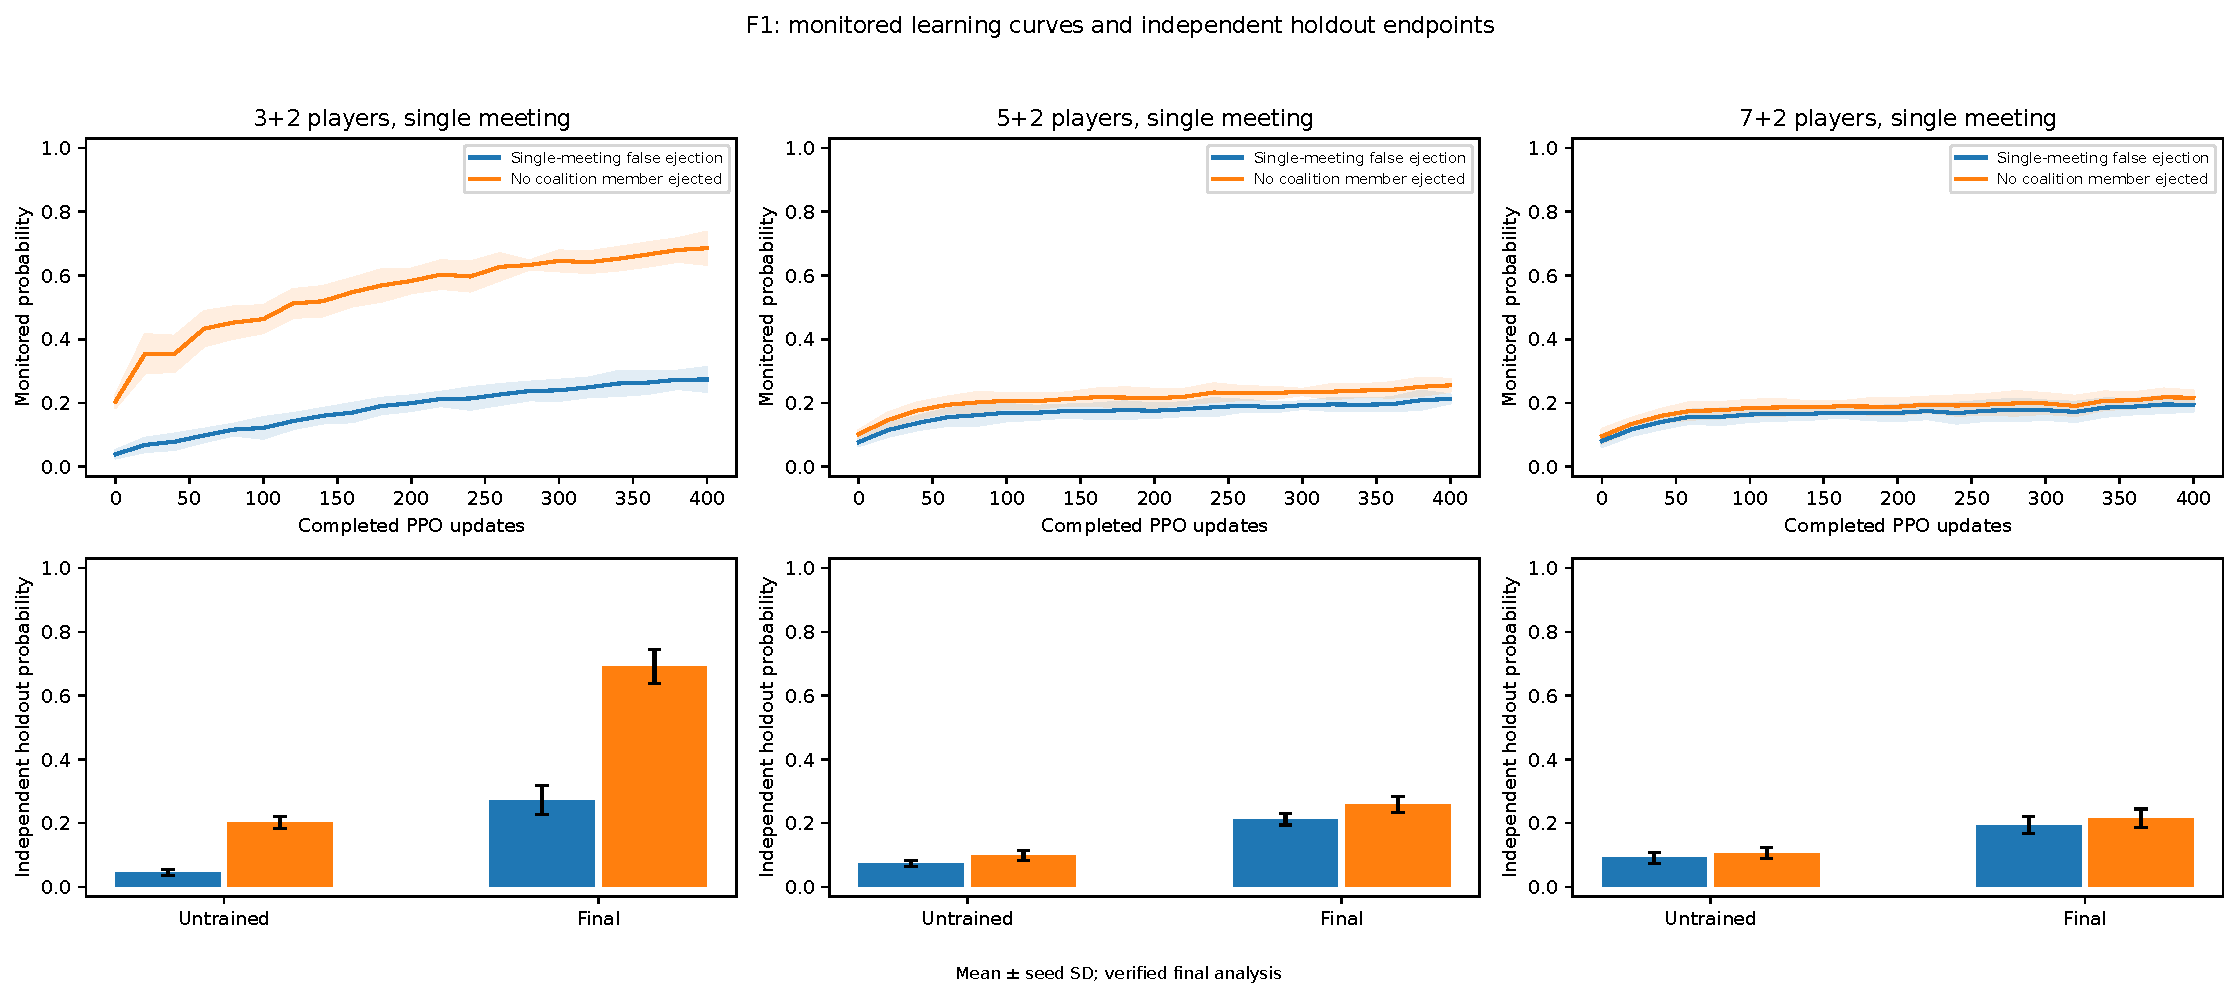
\includegraphics[width=1\linewidth,height=0.6\textheight]{figures/final/f1_learning_and_holdout.pdf}
\caption{Figure 1. Coalition learning against scripted soft-credibility
crew in the meeting-only game. Curves use monitored evaluations;
untrained and final points use independent holdout episodes. Variability
is across ten seeds. Vote agreement is raw; the false-claim denominator
includes non-informative actions.}\label{fig:1}
\end{figure}

\FloatBarrier

\subsection{Scripted performance and adaptive robustness
differ}\label{scripted-performance-and-adaptive-robustness-differ}

The seven-rule scripted comparison (F2) exposes an accuracy tradeoff. At
5+2, hypothesis scoring reduces false ejection relative to the mean
under alibi (0.1469 versus 0.3273) and framing (0.1542 versus 0.4106),
but increases it under the lone liar (0.1907 versus 0.1311). Its
truthful-testimony false-ejection rate is 0.3700, whereas mean and soft
credibility have zero observed errors (Figure 2). The corresponding
hypothesis errors at 3+2 and 7+2 are 0.2447 and 0.3926. Here
\emph{truthful} describes supported claim contents; information
selection and coalition voting remain adversarial.

\begin{figure}
\centering
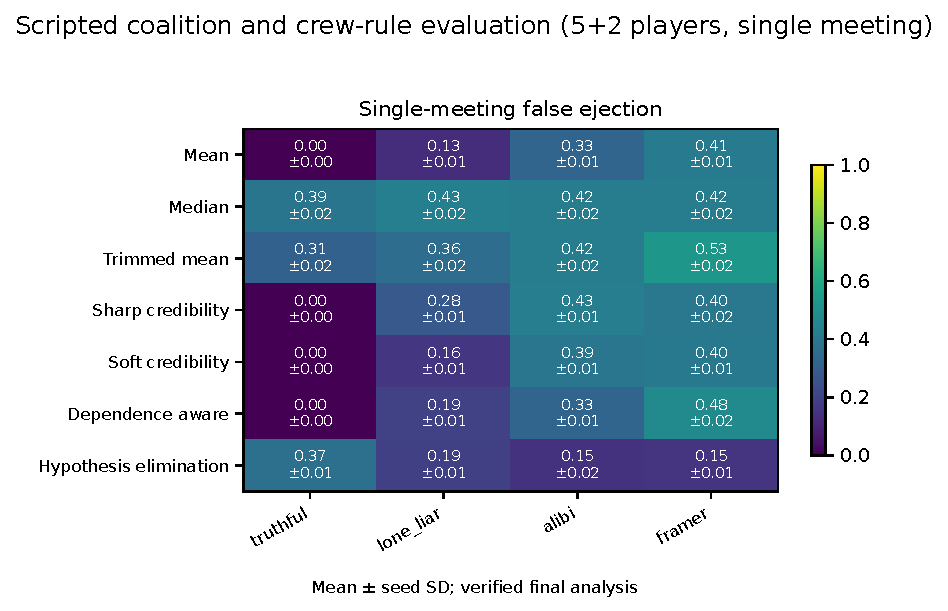
\includegraphics[width=1\linewidth,height=0.6\textheight]{figures/final/f2_tenseed_crew5_rules.pdf}
\caption{Figure 2. False-ejection rates for seven defenses against four
scripted coalitions at 5+2, with ten replicates and 1,000 episodes per
cell. Creator-ejection outcomes are available in the released data.
These descriptive comparisons retain the full F2 multiplicity
families.}\label{fig:2}
\end{figure}

Median and trimmed rules can discard useful sparse testimony, so
scalar-contamination robustness does not ensure accurate votes.
Hypothesis feasibility is also insufficient: a bounded replay of ten
truthful-testimony errors found that the true coalition retained
positive weight and its timelines satisfied the emitted constraints.
Some errors arose from exact score ties resolved by agent index; another
involved unanimous honest abstention. This replay identifies possible
failure routes, not their prevalence. Since skips do not compete in the
candidate tally, coalition ballots can decide an ejection when all
honest voters abstain. The 63- and 36-test F2 families cannot reject at
0.05 with the retained ten-seed exact-test resolution.

Targeted training against the hypothesis rule (F8) exposes a further
vulnerability. At 5+2, its false-ejection rate increases from 0.1255
against a soft-trained coalition to 0.4217 against a hypothesis-trained
coalition: paired effect 0.2962, pointwise 95\% CI {[}0.2521, 0.3418{]},
Holm-adjusted \(p=0.0273\). The hypothesis-trained/hypothesis-tested
pairing exceeds soft-trained/soft-tested false ejection by 0.2275
(\(p=0.0273\)). Yet the hypothesis-trained attack obtains only 0.0962
against mean and 0.0976 against soft credibility (Figure 3). The attack
specializes to its training defense. At 7+2 the hypothesis rate reaches
0.6036, a descriptive result based on five seeds.

\begin{figure}
\centering
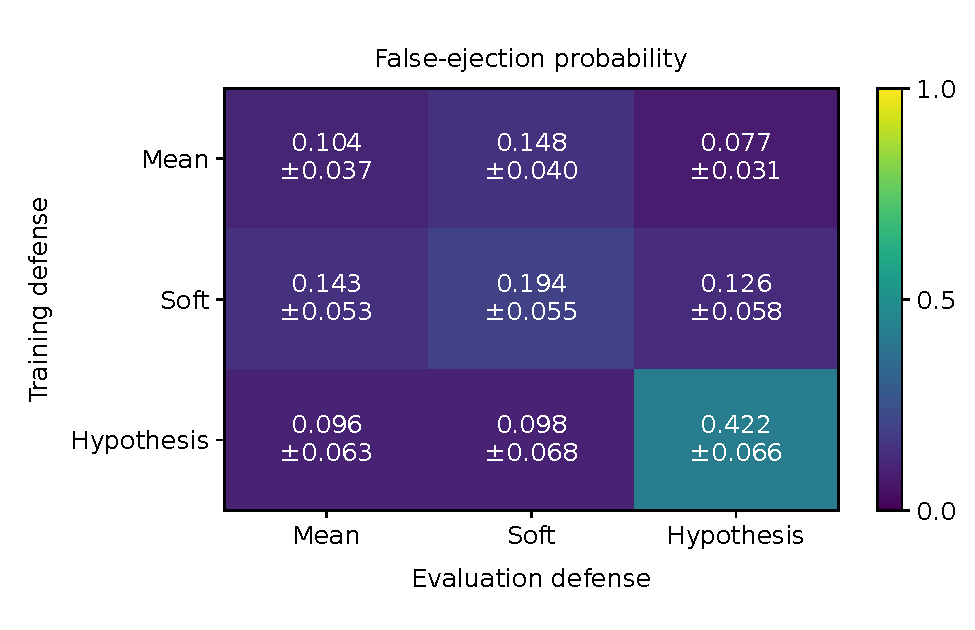
\includegraphics[width=1\linewidth,height=0.6\textheight]{figures/v2/hypothesis_crossplay.pdf}
\caption{Figure 3. False-ejection rates in adaptive hypothesis crossplay
at 5+2. Rows identify the coalition's training defense and columns its
evaluation defense; entries are mean ± sample SD across ten seeds with
1,000 final episodes per cell. The hypothesis-trained coalition
transfers poorly to the other two rules.}\label{fig:3}
\end{figure}

An independent 67,500-episode ballot study reproduces the elevated
hypothesis-attack error: 0.4240 at 5+2 and 0.6048 at 7+2. Honest voters
abstain at rates 0.6608 and 0.8988. Removing coalition ballots prevents
97.26\% and 100\% of observed false ejections; coalition ballots alone
suffice in 97.75\% and 100\%. Crew-only false ejection is 0.0142 and
zero, respectively. Table 2 compares attack types at 5+2. These are
fixed-ballot counterfactuals: they support an abstention-related route
to failure, but do not predict how agents would vote under a changed
rule or establish abstention as the only cause.

\FloatBarrier

\begin{table}[htbp]
\centering
\caption{Table 2. Independent ballot diagnostics against the hypothesis defender
at 5+2. Entries average within-seed rates over ten seeds. Necessary and
sufficient condition on observed false ejection and hold recorded votes
fixed; crew-only FE removes coalition ballots. Full precision, SDs, and
denominator counts are released with the data.}\label{tab:2}
\begin{tabular}{@{}
  >{\raggedright\arraybackslash}p{(\linewidth - 10\tabcolsep) * \real{0.1700}}
  >{\raggedleft\arraybackslash}p{(\linewidth - 10\tabcolsep) * \real{0.1100}}
  >{\raggedleft\arraybackslash}p{(\linewidth - 10\tabcolsep) * \real{0.1500}}
  >{\raggedleft\arraybackslash}p{(\linewidth - 10\tabcolsep) * \real{0.1800}}
  >{\raggedleft\arraybackslash}p{(\linewidth - 10\tabcolsep) * \real{0.1800}}
  >{\raggedleft\arraybackslash}p{(\linewidth - 10\tabcolsep) * \real{0.2100}}@{}}
\toprule\noalign{}
\begin{minipage}[b]{\linewidth}\raggedright
Attack
\end{minipage} & \begin{minipage}[b]{\linewidth}\raggedleft
FE
\end{minipage} & \begin{minipage}[b]{\linewidth}\raggedleft
Crew skip
\end{minipage} & \begin{minipage}[b]{\linewidth}\raggedleft
Necessary
\end{minipage} & \begin{minipage}[b]{\linewidth}\raggedleft
Sufficient
\end{minipage} & \begin{minipage}[b]{\linewidth}\raggedleft
Crew-only FE
\end{minipage} \\
\midrule\noalign{}

mean & 0.075 & 0.196 & 0.651 & 0.603 & 0.032 \\
soft & 0.117 & 0.271 & 0.684 & 0.662 & 0.040 \\
hypothesis & 0.424 & 0.661 & 0.973 & 0.978 & 0.014 \\
\bottomrule\noalign{}
\end{tabular}
\end{table}

\FloatBarrier

\subsection{Response training changes victory and voting harm
differently}\label{response-training-changes-victory-and-voting-harm-differently}

In spatial single-meeting crossplay (F3), unconditional false ejection
is more frequent against the learned defender. At 5+2, rates are 0.1940
for \(C_0\)--\(D_0\), 0.4031 for \(C_0\)--\(D_1\), and 0.5385 for
\(C_1\)--\(D_1\); the adapted coalition obtains only 0.0759 against
\(D_0\). The specified defender-effect contrast, \(C_0\)--\(D_0\) minus
\(C_0\)--\(D_1\), is negative at all three populations (adjusted
\(p=0.0176\)). Coalition adaptation against \(D_1\) is not uniformly
beneficial: its false-ejection effect is −0.0482 at 3+2, +0.1354 at 5+2,
and +0.1124 at 7+2; the negative effect does not reject.

The incident decomposition changes its interpretation. For
\(C_0\)--\(D_1\), total false-ejection probability equals
incident-associated plus incident-free false ejection: 0.4635 = 0.0202 +
0.4433 at 3+2, 0.4031 = 0.0903 + 0.3128 at 5+2, and 0.4747 = 0.1552 +
0.3195 at 7+2. Each component uses all games as its denominator; these
are joint, not incident-conditional, probabilities. At 5+2, incident
probability is 0.9626 against \(D_0\) but 0.2543 against \(D_1\). F3
rewards the defender +1 in incident-free games even after innocent
ejection. Most of its observed false ejections therefore occur outside
the reward's penalized conditions. Unconditional error alone cannot
establish greater vulnerability to deceptive testimony: the comparison
also changes incident opportunities and includes a reward--metric
mismatch. Indeed, the joint incident-and-false-ejection rate decreases
after defender training at all three populations; at 5+2 the overall
increase decomposes as \(0.2091 = -0.0775 + 0.2866\), with the increase
confined to incident-free games. Some 3+2 seeds have no incidents
against \(D_1\); their conditional rates remain undefined while
unconditional summaries retain all ten seeds.

Eight-round play (F4) optimizes terminal victory, while innocent
ejection is an additional evaluation outcome. Descriptive victory and
voting-harm rates differ (Figure 4). At 5+2, victory rates are 0.9670
(\(C_0\)--\(D_0\)), 0.3603 (\(C_0\)--\(D_1\)), and 0.8514
(\(C_1\)--\(D_1\)). The last adaptation raises victory by 0.4911 while
changing the probability of any innocent ejection only from 0.8392 to
0.8467 and reducing mean innocent-ejection count by 0.4249 per game. At
7+2, victory rises by 0.5104 while mean count falls by 1.0066.
Differently terminated or shorter games can therefore produce more
coalition wins with fewer total innocent ejections.

\begin{figure}
\centering
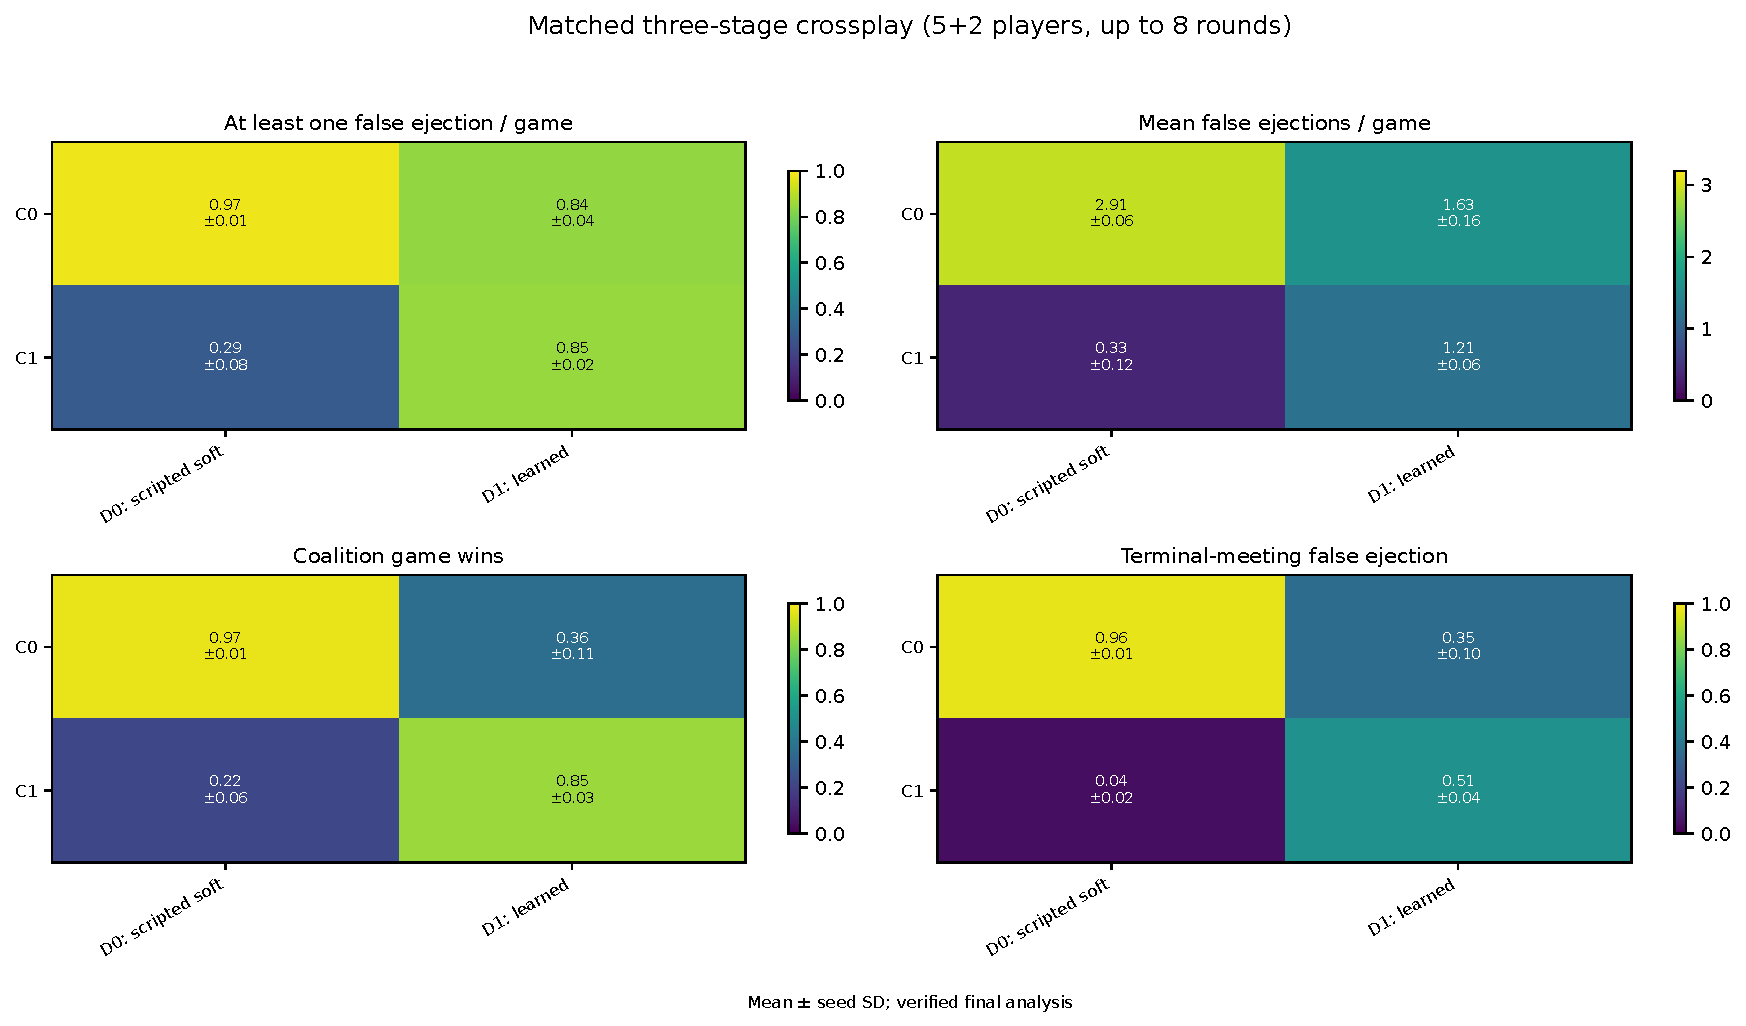
\includegraphics[width=1\linewidth,height=0.6\textheight]{figures/final/f4_tenseed_crew5_crossplay.pdf}
\caption{Figure 4. Eight-round crossplay at 5+2 across ten seeds.
Coalition victory, any innocent ejection, mean innocent-ejection count,
and terminal outcomes are distinct. Whole-game harm includes
incident-free meetings. The 27-contrast F4 family has no Holm rejection
at 0.05.}\label{fig:4}
\end{figure}

Transfer again depends on population: \(C_1\)--\(D_0\) wins 0.2182 at
5+2 and 0.0630 at 7+2, but 0.9882 at 3+2. All F4 effects are descriptive
under the retained family: its minimum attainable adjusted p-value is
0.0527. Large point estimates and pointwise intervals do not override
that familywise limitation.

\FloatBarrier

\subsection{Repeated responses produce finite, opponent-specific
gains}\label{repeated-responses-produce-finite-opponent-specific-gains}

Ten-generation crossplay (F5) shows renewed coalition gains against the
latest defender. In the separate 5+2 multi-round loop, coalition victory
is 0.9658 for \(C_0\)--\(D_0\), 0.3524 for \(C_0\)--\(D_1\), and 0.8562
for \(C_1\)--\(D_1\). At generation ten it is 0.3068 for
\(C_9\)--\(D_{10}\) and 0.7968 for \(C_{10}\)--\(D_{10}\), while
\(C_{10}\)--\(D_0\) achieves only 0.1804 (Figure 5). These values come
from the multi-generation evaluation, independently of F4.

\begin{figure}
\centering
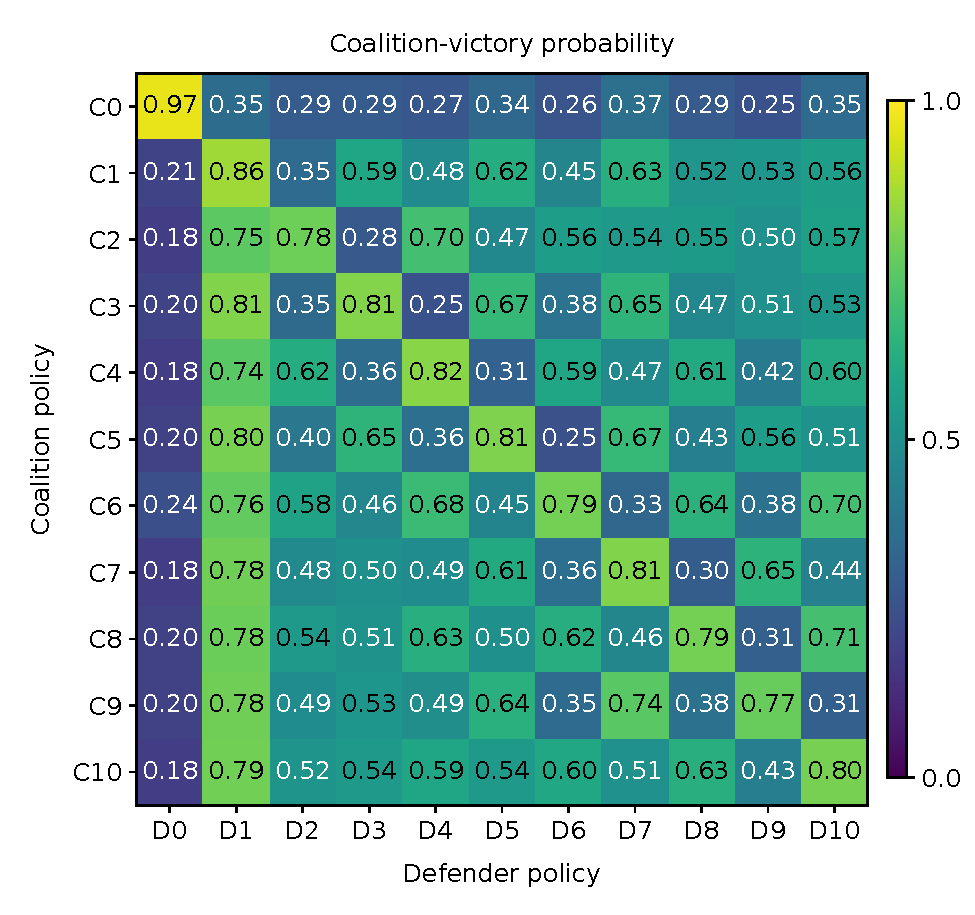
\includegraphics[width=1\linewidth,height=0.75\textheight]{figures/v2/finite_crossplay.pdf}
\caption{Figure 5. Coalition-victory rates in full ten-generation 5+2
crossplay, averaged across ten seeds with 500 episodes per cell. Each
diagonal entry minus the entry immediately above measures coalition
adaptation against a fixed defender. Poor transfer to earlier defenders
distinguishes these gains from a uniformly stronger
coalition.}\label{fig:5}
\end{figure}

Matrix gain averages \(M_{g,g}-M_{g-1,g}\) over response generations:
the outcome is false ejection for single-meeting loops and coalition
victory for multi-round loops. Mean gains are 0.300 in 5+2
single-meeting play, 0.501 in 5+2 multi-round play, and 0.576 in 3+2
multi-round play. Their tests pass Holm correction in the 25-test
dynamics family (\(p=0.0488\)). The shorter 7+2 loop has a descriptive
gain of 0.418 but only five seeds. No specified late-minus-early or
parity test rejects after correction. Policy distances and finite-pool
response gaps are retained in the released analysis; neither they nor
the observed alternation establish convergence, nonconvergence, optimal
responses, or an attracting cycle. Each stage starts from fresh weights
and faces a different frozen opponent.

\FloatBarrier

\subsection{Dependence penalties have conditional
benefits}\label{dependence-penalties-have-conditional-benefits}

Dependence-aware defenses (F7) do not show a general adaptive-attack
gain. At 5+2, training against the testimony-discount rule changes its
false-ejection rate from 0.1819 to 0.1696: effect −0.0123, CI
{[}−0.0516, 0.0374{]}, adjusted \(p=1\). Against the combined rule and
ballot discount, retraining changes 0.2044 to 0.1896: effect −0.0148, CI
{[}−0.0513, 0.0215{]}, adjusted \(p=1\). At 3+2, combined-defense error
instead rises descriptively from 0.4132 to 0.8722; five seeds preclude a
raw 0.05 rejection. None of these comparisons establishes immunity. The
static spatial rule sweep likewise shows attack-dependent rankings and
is distinct from F2's exogenous-evidence comparison.

In the four-generation 5+2 loop, dependence-aware defense increases any
innocent ejection by 0.042425 after coalition stages (CI {[}0.034775,
0.049400{]}) and by 0.104375 after defender stages ({[}0.073274,
0.135025{]}); both adjusted p-values are 0.0117. After coalition stages
it reduces coalition victory by 0.028775 ({[}−0.045625, −0.012050{]},
\(p=0.0410\)). Table 3 retains all six comparisons, including the
nonsignificant defender-stage victory result. Smaller adaptation gains
therefore coexist with greater voting harm.

\FloatBarrier

\begin{table}[htbp]
\centering
\caption{Table 3. Dependence-aware versus reference loops over the same four
generations and ten seeds. Values are means ± sample SD; differences are
defended minus reference, and stage summaries exclude \(C_0\). Holm
correction retains the complete six-comparison family.}\label{tab:3}
\begin{tabular}{@{}
  >{\raggedright\arraybackslash}p{(\linewidth - 10\tabcolsep) * \real{0.1800}}
  >{\raggedleft\arraybackslash}p{(\linewidth - 10\tabcolsep) * \real{0.1700}}
  >{\raggedleft\arraybackslash}p{(\linewidth - 10\tabcolsep) * \real{0.2000}}
  >{\raggedleft\arraybackslash}p{(\linewidth - 10\tabcolsep) * \real{0.2000}}
  >{\raggedleft\arraybackslash}p{(\linewidth - 10\tabcolsep) * \real{0.1400}}
  >{\raggedleft\arraybackslash}p{(\linewidth - 10\tabcolsep) * \real{0.1100}}@{}}
\toprule\noalign{}
\begin{minipage}[b]{\linewidth}\raggedright
Outcome
\end{minipage} & \begin{minipage}[b]{\linewidth}\raggedleft
Summary
\end{minipage} & \begin{minipage}[b]{\linewidth}\raggedleft
Reference
\end{minipage} & \begin{minipage}[b]{\linewidth}\raggedleft
Defended
\end{minipage} & \begin{minipage}[b]{\linewidth}\raggedleft
Difference
\end{minipage} & \begin{minipage}[b]{\linewidth}\raggedleft
Holm p
\end{minipage} \\
\midrule\noalign{}

Any FE & C stages & 0.847 ± 0.009 & 0.890 ± 0.007 & +0.042 & 0.0117 \\
Any FE & D stages & 0.658 ± 0.051 & 0.763 ± 0.047 & +0.104 & 0.0117 \\
Any FE & Matrix gain & 0.191 ± 0.051 & 0.129 ± 0.046 & -0.062 &
0.0234 \\
Coalition win & C stages & 0.817 ± 0.025 & 0.789 ± 0.026 & -0.029 &
0.0410 \\
Coalition win & D stages & 0.309 ± 0.065 & 0.348 ± 0.054 & +0.040 &
0.1387 \\
Coalition win & Matrix gain & 0.509 ± 0.086 & 0.445 ± 0.070 & -0.064 &
0.0469 \\
\bottomrule\noalign{}
\end{tabular}
\end{table}

\FloatBarrier

\subsection{Information, budget, and reward
controls}\label{information-budget-and-reward-controls}

The five-seed controls qualify the interpretation. Removing both the
private channel and partner feature gives initial-coalition
single-meeting false ejection 0.2518, versus 0.1854 by default. Shared
parameters, rewards, and possible role inference remain, so this does
not isolate every coordination mechanism or establish that explicit
communication is needed.

On matched seeds, extending defender training from 400 to 800 or 1,600
updates gives \(C_1\)--\(D_1\) single-meeting false ejection 0.5252,
0.5672, and 0.5160. Alternative rewards also change descriptive
adaptation gains: in the four-generation single-meeting loop, matrix
gains are 0.287 by default, 0.164 with balanced rewards for both sides,
and 0.220 with meeting rewards for both. In the two-generation
multi-round control, victory gains are 0.440 under survival and 0.333
under framing count. None of the nine outcome-ablation, eight budget, or
eighteen reward comparisons rejects after Holm correction. Five-seed
resolution and finite budgets prevent conclusions of equivalence or
optimal training.

\FloatBarrier

\section{Mechanisms: score construction and correlated
reports}\label{mechanisms-score-construction-and-correlated-reports}

The 540,000-episode mechanism study checks whether excessive total
coalition weight accompanies errors in the tested scripted records.
Under alibi attacks, soft credibility's mean coalition weight is 0.2630
at 3+2, 0.1425 at 5+2, and 0.0976 at 7+2, below the uniform shares
0.5000, 0.3333, and 0.2500. These shares count actual reporters after
the incident victim is removed. Across all 240,000 retained honest-voter
records, none exceeds its uniform share at tolerance \(10^{-12}\). This
result is specific to these scripted records.

Nevertheless, soft credibility increases alibi false ejection relative
to the mean by 0.0112, 0.0680, and 0.1586 across the three populations.
The score combines two relevant terms: witness alibis reduce suspicion,
while a caught liar's self-incriminating penalty sits inside that
speaker's downweighted row. Removing alibi credit, including the
positive was-with subject credit governed by the same coefficient,
reduces alibi errors for every tested rule and size. Moving the catch
penalty into private evidence reduces soft alibi false ejection by
0.0242, 0.0912, and 0.1750. These interventions match initial evidence
but allow responses and votes to change.

The benefits are conditional. Removing alibi credit increases soft
framer error by 0.0876 at 5+2 and 0.1332 at 7+2; moving the catch
penalty increases soft lone-liar error by 0.1540 at 3+2. Lower false
ejection can also mean more no-ejection outcomes: under 3+2 alibi
attacks, every tested variant has zero creator ejection and
coalition-favorable rate one, meaning no coalition member is ejected,
including meetings with no ejection. Under 5+2 lone liars, soft
catch-outside reduces false ejection from 0.1598 to 0.1316 but increases
coalition-favorable outcomes from 0.2000 to 0.2416. The narrow finding
is that these alibi errors occur without excessive total coalition
weight, while score modifications have condition-dependent effects.
Because responses and votes change with the interventions, they do not
isolate a unique causal channel or localize all failures to candidate
scoring.

The Gaussian model (F6) isolates weight amplification under different
assumptions. There are \(n\) honest reports with independent
variance-\(\sigma^2\) Gaussian noise, and \(m<n\) coalition reports with
bias \(b\), marginal variance \(\sigma_c^2\), and equicorrelation
\(\rho\). Reports within distance \(h\) corroborate one another; weights
are proportional to \(e^{\gamma c_i}\), where \(c_i\) counts
corroboration. Replacing counts by their expectations defines the
surrogate coalition weight

\[
W_C=\frac{f}{f+(1-f)e^{-\gamma\Delta c}},\qquad
f=\frac{m}{n+m},\quad \Delta c=\bar c_C-\bar c_H.
\]

For \(\gamma>0\), amplification \(W_C>f\) occurs exactly when
\(\Delta c>0\). The median instead has a uniform error bound in
coalition bias when \(m<n\). A long-window dependence penalty can make
surrogate coalition weight non-increasing with correlation on a
specified branch; Appendix A gives the assumptions, threshold, and
proof. The amplification and dependence claims concern the surrogate.
For example, with \(n=5\), \(m=2\), equal unit variances, \(b=20\),
\(h=0.43\), \(\rho=\gamma=1\), it predicts \(W_C=0.295>2/7\), while
100,000 Monte Carlo trials give mean realized weight 0.277, below the
uniform share.

The numerical report and sensor examples remain illustrative. For the
report model at
\(n=5,m=2,h=0.4\sigma,b=4\sigma,\sigma_c=\sigma,\gamma=1\), credibility
MSE in units of \(\sigma^2\) changes from 0.87 with independent
coalition noise to 1.84 with perfectly correlated noise. The
dependence-aware rule gives 0.31 in the correlated case but 1.02 in the
independent case. In the twelve-sensor analogue with three coordinated
compromised sensors, credibility RMSE is \(0.99\sigma\), versus
\(0.83\sigma\) for the mean, \(0.58\sigma\) for the median, and
\(0.56\sigma\) for the dependence variant across twenty runs. These
parameter-specific benefits do not establish a general repair. The model
omits the game's alibi credit and catch penalties, and its
reporter-minority condition excludes the 2+2 electorate remaining after
an incident in the initial 3+2 game.

\FloatBarrier

\section{Discussion and limitations}\label{discussion-and-limitations}

Three distinctions organize the findings. Scripted performance differs
from adaptive crossplay; victory differs from voting harm; and an
observed scoring intervention differs from identifying a causal
mechanism. F3 leaves incident-free ejections unpenalized, while F4
optimizes victory rather than innocent-ejection avoidance. These
reward--metric mismatches limit a simple interpretation of increased
harm as failed resistance to deception. Raw vote agreement under shared
parameters and incentives also does not establish communication-driven
collusion. Adaptive crossplay and direct diagnostics characterize these
outcomes without resolving those causal questions.

The scope is limited by the benchmark and learning procedure. Small
maps, structured claims, and two policy-sharing impostors do not
establish behavior in natural-language deliberation or independently
incentivized coalitions. Non-recurrent actors retain limited cross-round
memory. Fresh initialization, finite PPO budgets, and a restricted
policy pool preclude claims about optimal responses or asymptotic
dynamics. The hypothesis rule's deterministic ties, constraint
relaxations, and uncalibrated scores also limit what its vulnerability
establishes about stronger inference-based defenses.

Statistical resolution is a material limitation, not evidence that small
studies establish equivalence. The five-seed and large-family
restrictions described in Methods apply even to large point estimates.
The mechanism interventions preserve initial evidence rather than full
transcripts; ballot removal preserves votes rather than behavior. These
limits prevent unique causal explanations or universal defense rankings.
Several implementation repairs changed together, so differences from
historical runs cannot identify one repair's effect. The released
protocols and raw records make the reported comparisons auditable.

\FloatBarrier

\section{Conclusion}\label{conclusion}

Training is associated with higher false-ejection rates and raw
coalition vote agreement; it does not establish communication-driven
collusion or greater truthfulness. Hypothesis scoring combines
scripted-attack benefits with baseline error and targeted vulnerability.
Finite response sequences show opponent-specific gains, while victory
and innocent harm can differ under objectives that do not penalize every
measured harm. These exploratory findings motivate adaptive-defense
crossplay, separate outcome reporting, and direct diagnostics, without
establishing a universal causal mechanism or a permanent learning cycle.

\FloatBarrier

\section*{Acknowledgements}\label{acknowledgements}
\addcontentsline{toc}{section}{Acknowledgements}

OpenAI Codex, using GPT-6, assisted with implementation review,
correction and testing of research code, numerical reanalysis, and
manuscript editing. Numerical measurements were produced by the
executable experiments and analysis scripts described in this paper.

\FloatBarrier

\section*{Data availability}\label{data-availability}
\addcontentsline{toc}{section}{Data availability}

Code, complete seed-level summaries, all planned comparisons, and
diagnostic tables are available in
\href{https://github.com/IsaacLin247/coalition-deception}{Coalition
Deception}. The
\href{https://github.com/IsaacLin247/coalition-deception/releases/tag/corrected-study-2026-09-11}{corrected-study-2026-09-11
release} contains the frozen source, checkpoints, raw episode and
meeting records, environment manifests, and checksums. Appendix B
describes reproduction. The complete numerical grids and extended
figures remain available there, including comparisons summarized in this
article.

\FloatBarrier

\section*{References}\label{references}
\addcontentsline{toc}{section}{References}

\protect\phantomsection\label{refs}
\begin{CSLReferences}{0}{0}
\bibitem[\citeproctext]{ref-crawford1982}
\CSLLeftMargin{{[}1{]} }%
\CSLRightInline{V. P. Crawford and J. Sobel, {``Strategic information
transmission,''} \emph{Econometrica}, vol. 50, no. 6, pp. 1431--1451,
1982, doi: \href{https://doi.org/10.2307/1913390}{10.2307/1913390}.}

\bibitem[\citeproctext]{ref-lewis1969}
\CSLLeftMargin{{[}2{]} }%
\CSLRightInline{D. Lewis, \emph{Convention: A philosophical study}.
Harvard University Press, 1969.}

\bibitem[\citeproctext]{ref-kharitonov2019}
\CSLLeftMargin{{[}3{]} }%
\CSLRightInline{E. Kharitonov, R. Chaabouni, D. Bouchacourt, and M.
Baroni, {``{EGG}: A toolkit for research on emergence of lanGuage in
games,''} in \emph{Proceedings of the 2019 conference on empirical
methods in natural language processing and the 9th international joint
conference on natural language processing: System demonstrations}, 2019,
pp. 55--60. doi:
\href{https://doi.org/10.18653/v1/D19-3010}{10.18653/v1/D19-3010}.}

\bibitem[\citeproctext]{ref-condorelli2024}
\CSLLeftMargin{{[}4{]} }%
\CSLRightInline{D. Condorelli and M. Furlan, {``Cheap talking
algorithms.''} 2024. Available:
\url{https://arxiv.org/abs/2310.07867v6}}

\bibitem[\citeproctext]{ref-chen2025}
\CSLLeftMargin{{[}5{]} }%
\CSLRightInline{K. Chen, {``Communication with multiple senders.''}
2025. Available: \url{https://arxiv.org/abs/2505.14639v1}}

\bibitem[\citeproctext]{ref-arieli2023}
\CSLLeftMargin{{[}6{]} }%
\CSLRightInline{I. Arieli, I. Geffner, and M. Tennenholtz, {``Resilient
information aggregation,''} in \emph{Proceedings of the 19th conference
on theoretical aspects of rationality and knowledge (TARK)}, in
Electronic proceedings in theoretical computer science, vol. 379. 2023,
pp. 31--45. doi:
\href{https://doi.org/10.4204/EPTCS.379.6}{10.4204/EPTCS.379.6}.}

\bibitem[\citeproctext]{ref-figura2021}
\CSLLeftMargin{{[}7{]} }%
\CSLRightInline{M. Figura, Y. Lin, J. Liu, and V. Gupta, {``Resilient
consensus-based multi-agent reinforcement learning with function
approximation.''} 2021. Available:
\url{https://arxiv.org/abs/2111.06776}}

\bibitem[\citeproctext]{ref-witkowski2012}
\CSLLeftMargin{{[}8{]} }%
\CSLRightInline{J. Witkowski and D. C. Parkes, {``A robust {B}ayesian
truth serum for small populations,''} in \emph{Proceedings of the 26th
AAAI conference on artificial intelligence}, 2012, pp. 1492--1498. doi:
\href{https://doi.org/10.1609/aaai.v26i1.8261}{10.1609/aaai.v26i1.8261}.}

\bibitem[\citeproctext]{ref-elmhamdi2023}
\CSLLeftMargin{{[}9{]} }%
\CSLRightInline{E.-M. El-Mhamdi, S. Farhadkhani, R. Guerraoui, and L.-N.
Hoang, {``On the strategyproofness of the geometric median,''} in
\emph{Proceedings of the 26th international conference on artificial
intelligence and statistics (AISTATS)}, in Proceedings of machine
learning research, vol. 206. 2023, pp. 2603--2640. Available:
\url{https://proceedings.mlr.press/v206/el-mhamdi23a.html}}

\bibitem[\citeproctext]{ref-kopparapu2022}
\CSLLeftMargin{{[}10{]} }%
\CSLRightInline{K. Kopparapu \emph{et al.}, {``Hidden agenda: A social
deduction game with diverse learned equilibria.''} 2022. Available:
\url{https://arxiv.org/abs/2201.01816}}

\bibitem[\citeproctext]{ref-sarkar2025}
\CSLLeftMargin{{[}11{]} }%
\CSLRightInline{B. Sarkar, W. Xia, C. K. Liu, and D. Sadigh, {``Training
language models for social deduction with multi-agent reinforcement
learning,''} in \emph{Proceedings of the 24th international conference
on autonomous agents and multiagent systems (AAMAS)}, 2025, pp.
1830--1839. doi:
\href{https://doi.org/10.65109/PHJJ9903}{10.65109/PHJJ9903}.}

\bibitem[\citeproctext]{ref-blumenkamp2021}
\CSLLeftMargin{{[}12{]} }%
\CSLRightInline{J. Blumenkamp and A. Prorok, {``The emergence of
adversarial communication in multi-agent reinforcement learning,''} in
\emph{Proceedings of the 2020 conference on robot learning}, in
Proceedings of machine learning research, vol. 155. 2021, pp.
1394--1414. Available:
\url{https://proceedings.mlr.press/v155/blumenkamp21a.html}}

\bibitem[\citeproctext]{ref-li2021}
\CSLLeftMargin{{[}13{]} }%
\CSLRightInline{J. Li \emph{et al.}, {``Shapley counterfactual credits
for multi-agent reinforcement learning,''} in \emph{Proceedings of the
27th ACM SIGKDD conference on knowledge discovery and data mining},
2021, pp. 934--942. doi:
\href{https://doi.org/10.1145/3447548.3467420}{10.1145/3447548.3467420}.}

\bibitem[\citeproctext]{ref-orzan2024}
\CSLLeftMargin{{[}14{]} }%
\CSLRightInline{N. Orzan, E. Acar, D. Grossi, and R. Rădulescu,
{``Emergent cooperation under uncertain incentive alignment,''} in
\emph{Proceedings of the 23rd international conference on autonomous
agents and multiagent systems (AAMAS)}, 2024, pp. 1521--1530. Available:
\url{https://arxiv.org/abs/2401.12646}}

\bibitem[\citeproctext]{ref-motwani2024}
\CSLLeftMargin{{[}15{]} }%
\CSLRightInline{S. R. Motwani \emph{et al.}, {``Secret collusion among
{AI} agents: Multi-agent deception via steganography,''} in
\emph{Advances in neural information processing systems 37 (NeurIPS)},
2024. doi:
\href{https://doi.org/10.52202/079017-2336}{10.52202/079017-2336}.}

\bibitem[\citeproctext]{ref-tramer2020}
\CSLLeftMargin{{[}16{]} }%
\CSLRightInline{F. Tramèr, N. Carlini, W. Brendel, and A. Madry, {``On
adaptive attacks to adversarial example defenses,''} in \emph{Advances
in neural information processing systems}, 2020. Available:
\url{https://arxiv.org/abs/2002.08347}}

\bibitem[\citeproctext]{ref-lanctot2017}
\CSLLeftMargin{{[}17{]} }%
\CSLRightInline{M. Lanctot \emph{et al.}, {``A unified game-theoretic
approach to multiagent reinforcement learning,''} in \emph{Advances in
neural information processing systems}, 2017. Available:
\url{https://arxiv.org/abs/1711.00832}}

\bibitem[\citeproctext]{ref-schulman2017}
\CSLLeftMargin{{[}18{]} }%
\CSLRightInline{J. Schulman, F. Wolski, P. Dhariwal, A. Radford, and O.
Klimov, {``Proximal policy optimization algorithms.''} 2017. Available:
\url{https://arxiv.org/abs/1707.06347}}

\bibitem[\citeproctext]{ref-huang2022}
\CSLLeftMargin{{[}19{]} }%
\CSLRightInline{S. Huang and S. Ontañón, {``A closer look at invalid
action masking in policy gradient algorithms,''} in \emph{Proceedings of
the international FLAIRS conference}, 2022. doi:
\href{https://doi.org/10.32473/flairs.v35i.130584}{10.32473/flairs.v35i.130584}.}

\end{CSLReferences}

\FloatBarrier

\section*{Appendix A. Proposition: corroboration capture under
correlated
testimony}\label{appendix-a.-proposition-corroboration-capture-under-correlated-testimony}
\addcontentsline{toc}{section}{Appendix A. Proposition: corroboration
capture under correlated testimony}

\textbf{Setting.} Let \(1\le m<n\), \(N=n+m\), \(f=m/N\),
\(\sigma,\sigma_c,h>0\), \(\gamma,\lambda\ge0\), and \(\rho\in[0,1]\).
Honest reports are \(x_i=\theta+\varepsilon_i\) with independent
\(\varepsilon_i\sim\mathcal N(0,\sigma^2)\). Coalition reports are
\(y_j=\theta+b+\eta_j\), with
\(\eta\sim\mathcal N(0,\sigma_c^2[(1-\rho)I+\rho\mathbf1\mathbf1^\top])\),
independent of the honest noise. Define \(r=(x,y)\),
\(c_i=\#\{k\ne i:|r_i-r_k|\le h\}\), and the realized estimator
\(\hat\theta_{\rm cred}=\sum_i w_i r_i\), \(w_i\propto e^{\gamma c_i}\).
Dependence-aware weights additionally multiply by
\(e^{-\lambda\mathrm{ex}_i}\), where
\(\mathrm{ex}_i=\max_{k\ne i}D_{ik}-(N-1)^{-1}\sum_{k\ne i}D_{ik}\) and
\(D_{ik}\) is the agreement frequency across \(T\) independent
repetitions with fixed model parameters.

\textbf{Exact agreement probabilities.} With
\(s^2=\sigma^2+\sigma_c^2\), \[
p_{HH}=\operatorname{erf}(h/(2\sigma)),\qquad
p_{CC}(\rho)=\operatorname{erf}\!\left(\frac{h}{2\sigma_c\sqrt{1-\rho}}\right),\quad p_{CC}(1)=1,
\] \[
p_{HC}=\Phi((h-b)/s)-\Phi((-h-b)/s).
\] Hence \(\bar c_H=(n-1)p_{HH}+mp_{HC}\),
\(\bar c_C=(m-1)p_{CC}+np_{HC}\) and \(\Delta c=\bar c_C-\bar c_H\) is
non-decreasing in \(\rho\).

\textbf{Deterministic mean-field surrogate.} Replace each random
corroboration count by its group expectation. The resulting coalition
weight and estimator are \[
W_C=\frac{f}{f+(1-f)e^{-\gamma\Delta c}},\qquad
\tilde\theta=(1-W_C)\bar x+W_C\bar y.
\] This substitution defines a surrogate. In general
\(W_C\ne\mathbb E[\sum_{j\in C}w_j]\), and it does not give an exact
boundary for the realized estimator. Its exact bias and mean-squared
error are \[
\operatorname{bias}(\tilde\theta)=W_Cb,\qquad
\operatorname{MSE}(\tilde\theta)=W_C^2b^2+(1-W_C)^2\frac{\sigma^2}{n}
+W_C^2\sigma_c^2\left(\rho+\frac{1-\rho}{m}\right).
\] The approximation
\(\operatorname{MSE}(\tilde\theta)\approx W_C^2b^2\) requires the
displayed variance terms to be negligible relative to \(W_C^2b^2\).

\textbf{Proposition (surrogate amplification and robustness).}

\begin{enumerate}
\def\labelenumi{\arabic{enumi}.}
\item
  \emph{Weight amplification.} For \(\gamma>0\), \(W_C>f\) if and only
  if \(\Delta c>0\), equivalently \[
  (m-1)p_{CC}>(n-1)p_{HH}-(n-m)p_{HC}.
  \] At \(\gamma=0\), \(W_C=f\). When \(\Delta c>0\), \(W_C\) increases
  with \(\gamma\) and is non-decreasing in \(\rho\); \(W_C>1/2\)
  precisely when \(\gamma\Delta c>\log((1-f)/f)\). Weight amplification
  increases the surrogate's squared bias for \(b\ne0\); a comparison of
  total MSE must also include the variance terms above. At \(\rho=1\)
  and negligible cross-group agreement, the amplification condition
  reduces to \((m-1)>(n-1)p_{HH}\). Negligible cross-group agreement
  requires separation relative to the noise scale, for example
  \((|b|-h)/s\gg1\).
\item
  \emph{Median robustness and the bias reference.} Because \(m<n\), the
  pooled median \(M\) lies between the smallest and largest honest
  reports for every realization, irrespective of the coalition reports.
  Therefore \[
  \operatorname{MSE}(M)\le\sigma^2\mathbb E\!\left[\max_{1\le i\le n}|Z_i|^2\right]<\infty,
  \qquad Z_i\stackrel{\rm iid}{\sim}\mathcal N(0,1),
  \] uniformly in \(b\) and \(\rho\). For odd \(N\), writing
  \(k=(N+1)/2\) and \(Z_{(j)}\) for honest order statistics gives the
  sharper pathwise bound \(x_{(k-m)}\le M\le x_{(k)}\), hence
  \(|\operatorname{bias}(M)|\le\sigma\mathbb E[Z_{(k)}]\). As \(n,m\)
  grow with \(m/N\to f<1/2\), the latter upper bound tends to
  \(B_\infty=\sigma\Phi^{-1}(1/[2(1-f)])\). Thus \(W_C|b|=B_\infty\)
  defines an asymptotic bias-comparison reference, not a finite-sample
  MSE break-even boundary. For \(0<W^*=B_\infty/|b|<1\),
  \(W_C|b|>B_\infty\) is equivalent to \[
  \gamma\Delta c>\log\!\frac{(1-f)W^*}{f(1-W^*)}.
  \] When \(\Delta c>0\) and the right-hand side is positive, division
  by \(\Delta c\) gives the positive reference gain \(\gamma^*\).
  Finite-sample error comparisons use the actual risks or the
  finite-sample bound above. At \(f=1/2\), the median loses its uniform
  bound against arbitrarily displaced coalition reports; this does not
  imply that every estimator fails on every distribution.
\item
  \emph{Dependence penalty.} In the long-window limit, for \(m\ge2\), \[
  \overline{\mathrm{ex}}_C=\max(p_{CC},p_{HC})-\frac{(m-1)p_{CC}+np_{HC}}{N-1},
  \] \[
  \overline{\mathrm{ex}}_H=\max(p_{HH},p_{HC})-\frac{(n-1)p_{HH}+mp_{HC}}{N-1}.
  \] For \(m=1\), \(\overline{\mathrm{ex}}_C=0\) and coalition
  correlation has no effect. The defended surrogate replaces
  \(\gamma\Delta c\) by
  \(\gamma\Delta c-\lambda(\overline{\mathrm{ex}}_C-\overline{\mathrm{ex}}_H)\).
  On any correlation interval where \(m\ge2\) and
  \(p_{CC}(\rho)\ge p_{HC}\), its log-weight advantage depends on
  \(\rho\) through \[
  \left[\gamma(m-1)-\lambda\frac{n}{N-1}\right]p_{CC}(\rho).
  \] Consequently \(\lambda\ge\gamma(m-1)(N-1)/n\) makes the defended
  surrogate weight non-increasing with correlation on that interval; a
  strict inequality makes it decrease where \(p_{CC}\) increases. For
  \(5+2\), the threshold is \(1.2\gamma\). If \(p_{CC}<p_{HC}\), the
  coefficient instead is \((m-1)[\gamma+\lambda/(N-1)]\), so the stated
  repair condition does not apply there. A comparison between \(\rho=0\)
  and \(\rho=1\) requires the first branch to hold throughout that
  interval.
\end{enumerate}

\emph{Proof sketch.} Groupwise softmax normalization gives \(W_C\), and
independence of the two groups gives the exact surrogate variance. The
amplification and majority statements follow by rearranging the logistic
expression. Fewer than half the reports are adversarial, so neither
central rank can escape the honest range; for odd \(N\) at most \(m\)
insertions can shift the median's honest rank, giving the stated
order-statistic bounds. Gaussian symmetry gives the bias bound, and
convergence of central order statistics gives its fixed-fraction limit.
Finally, the strong law applied to each pair's agreement indicators
gives the long-window matrix entries. Taking each row's actual maximum
and collecting coefficients in \(p_{CC}\) yields the two dependence
branches. \(\square\)

\FloatBarrier

\section*{Appendix B. Implementation and
reproduction}\label{appendix-b.-implementation-and-reproduction}
\addcontentsline{toc}{section}{Appendix B. Implementation and
reproduction}

The original 82-file executable/configuration snapshot is identified by
SHA-256
691f7687435424185064b24a9fee1832c6e7b32b9661efe20a10e35ca0c17d35. The
portable package records its separate fingerprint while preserving the
scientific engine and 240 job designs. Original outputs retain their
original protocol identity. Complete configurations, action definitions,
scripts, and analysis commands accompany the public code and release;
the standard PPO and evaluation settings are given in Methods.

For scripted suspicion, private evidence scores scene sightings +3.0,
sightings elsewhere −3.5, unplaced agents +1.0, and non-informative
speakers +0.4. Testimony scores a caught lie +4.0 on its speaker,
self-contradiction +3.0, scene placement +1.5, witness alibi −2.0,
self-alibi −0.5, positive was-with claims −1.5 on the subject and −0.5
on the speaker, accusation +0.8, and contradiction +0.4. Voting requires
suspicion above 0.5. Hypothesis votes use the separate feasibility and
tie-breaking procedure in Methods.

The archive retains 11,885 checkpoints, including untrained,
intermediate, and final weights. Checks cover source and configuration
identities, finite architecture-compatible tensors, completed update
budgets, matching final checkpoints, raw episode/meeting outcomes, and
exact seed cohorts. All 303 contrasts in 15 families remain available,
including those summarized here. Operating systems and PyTorch builds
need not yield bit-identical training.

The mechanism records include 540,000 episodes and 240,000 honest-voter
views. The ballot records include 135 cells, 67,500 episodes, and
317,670 honest score views. Verification reconstructs the full
pre-ejection electorate, abstention, and ballot necessity/sufficiency.
Two terminal-coordination cells in the 7+2 loop are undefined because a
coalition voter was already lost in every game; the primary outcomes
remain complete, with no seed removed or undefined rate replaced by
zero. Mean catch-outside differs from its algebraically equal baseline
in two 3+2 alibi episodes because a \(2.22\times10^{-16}\) score
difference resolves an argmax tie; this does not support a substantive
intervention effect for the mean.

This single-document edition is built from \texttt{paper\_v2.md} by
\texttt{build\_v2.sh}, which generates standalone TeX and PDF with
Pandoc and XeLaTeX. The accompanying source manifest and verifier check
the retained numerical tables, figure identities, citations, and
original-manuscript preservation. Full numerical grids and extended
diagnostics remain in the public analysis.

\end{document}
